\documentclass[12pt]{article}
%\nonstopmode %Debug: Evita erros de packages nao inclusos

%Codificacao do arquivo e acentos
\usepackage[T1]{fontenc}
\usepackage[utf8]{inputenc}
\usepackage[brazilian]{babel}

%Fonte e formatacao de paragrafos
\usepackage{times}
\usepackage{indentfirst}
\usepackage{setspace}

%Pacote para carregar imagens
\usepackage{graphicx}

%Margens e formatacao de pagina
\usepackage{geometry}
\geometry{a4paper, total={210mm,297mm}, left=30mm, right=20mm, top=30mm, bottom=20mm}

\begin{document}

	%Capa do relatorio
	\begin{titlepage}
		\begin{center}
			{\fontsize{16pt}{\baselineskip}\fontfamily{\familydefault}\selectfont MATHEUS GIARETTA CANSIAN}\\[6cm]
			{\fontsize{18pt}{\baselineskip}\fontfamily{\familydefault}\selectfont \bf RELATÓRIO DE ESTÁGIO CURRICULAR}\\[5.5cm]
		\end{center}
		
		{
			\fontsize{14pt}{\baselineskip} \fontfamily{\familydefault} \selectfont
			
			\hspace{.45\textwidth} \begin{minipage}{.5\textwidth}
				\noindent 
				Relatório apresentado ao Curso de Engenharia Mecânica do Centro de Ciências Tecnológicas, 
				da Universidade do Estado de Santa Catarina, 
				como requisito parcial para a obtenção do grau de Bacharel em Engenharia Mecânica\\[0.6cm]
				Orientador: Fernando Hummel Lafratta\\[0.1cm]
				Supervisor: Michael Thamm
			\end{minipage}
		}\\[2.5cm]
		
		
		\begin{center}
		{
			\fontsize{14pt}{\baselineskip} \fontfamily{\familydefault} \selectfont
			Joinville, SC\\[0.2cm]
			2014
		}
		\end{center}
	\end{titlepage}

%Espacamento 1.5
\onehalfspacing

%Sumario
\tableofcontents
\pagebreak

%Lista de figuras
\listoffigures
\pagebreak

\section{Resumo}
\pagebreak

\section{Abstract}
\pagebreak


\section{Introdução}
	Este relatório é referente ao estágio obrigatório realizado pelo aluno Matheus Giaretta Cansian no curso de Bacharelado em Engenharia Mecânica da instituição UDESC de Joinville.
	O período no qual o estagiário atuou foi de 11 de abril de 2014 a 31 de dezembro de 2014, na empresa Husqvarna Construction Products, na cidade de Niederstotzingen, Alemanha.
\pagebreak

\section{Apresentação da concedente}

A Husqvarna é líder global em equipamentos para manejo de florestas, gramados e cuidado com o jardim. O grupo tambem é líder na Europa em produtos para irrigação residencial e um dos líderes mundiais em equipamentos para corte e ferramentas de diamante para a indústria da construção civil. As soluções desenvolvidas pelo grupo chegam ao mercado principalmente através de revendedores, tanto para uso doméstico quanto profissional. A Husqvarna está presente em mais de 100 paises com 14 mil funcionários e um faturamento anual de 4 bilhões do dólares.

\subsection{Marcas}
	Para atingir grupos distintos de consumidores a empresa não só utiliza a marca Husqvarna, como também outras, sendo Husqvarna, Gardena, McCulloch e Diamant Boart as principais marcas do Grupo.

\subsubsection{Husqvarna}

\begin{figure}[h!]
	\centering
	
\includegraphics[width=0.4\textwidth]{img/logo-husqvarna.png}
	\caption{Husqvarna}
\end{figure}

	Husqvarna é, há muitos anos, uma marca premium e forte em todo o mundo, representando a liderança tecnológica, desempenho profissional, alta qualidade e foco no usuário. A marca Husqvarna é responsável por aproximadamente 50\% das vendas do Grupo.

\subsubsection{Gardena}

\begin{figure}[h!]
	\centering
	
\includegraphics[width=0.4\textwidth]{img/logo-gardena.png}
	\caption{Gardena}
\end{figure}

	Gardena é a marca premium do canal varejo, líder na Europa em produtos para irrigação e ferramentas de jardim para o uso doméstico. A linha também inclui produtos movidos à bateria e representa aproximadamente 10\% das vendas do Grupo.

\subsubsection{McCulloch e Diamant Boart}

\begin{figure}[h!]
	\centering
	
\includegraphics[width=0.4\textwidth]{img/logo-mcdb.png}
	\caption{McCulloch e Diamant Boart}
\end{figure}

	McCulloch é uma marca premium global, incluindo produtos para manejo de florestas e jardins para consumidores exigentes do canal de varejo. 
	Diamant Boart é reconhecida como a marca líder global na indústria de pedras. A oferta de produtos inclui uma linha completa de ferramentas diamantadas para o processamento de pedra natural.	

\subsection{Visao}
	Vislumbramos um mundo onde as pessoas possam desfrutar de jardins, parques e florestas bem cuidados e experimentar estradas e edifícios refinados.

\subsection{Misao}
	Fornecemos soluções e produtos inovadores e de qualidade para tornar mais fácil o cuidado de jardins, parques e florestas, bem como as atividades do setor de construção, para profissionais e consumidores ao redor do mundo.

\begin{figure}[h!]
	\centering
	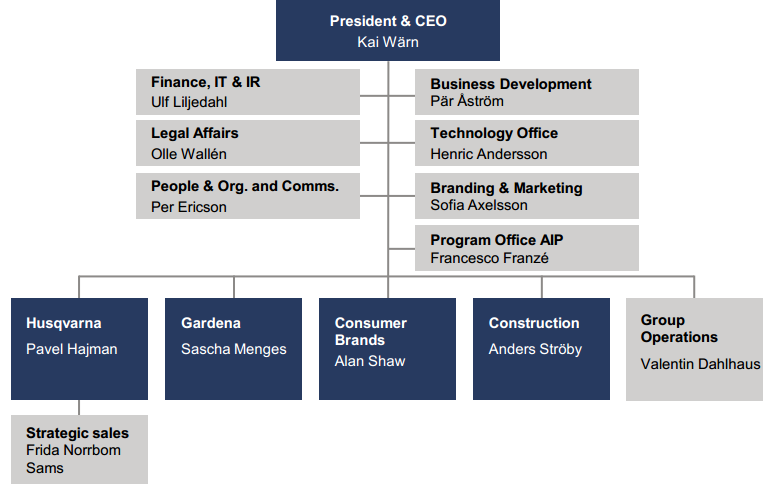
\includegraphics[width=0.9\textwidth]{img/organograma.png}
	\caption{Organograma da empresa}
	\label{organograma}
\end{figure}

%Construction é responsavel por 10\% do faturamento do grupo
	
\subsection{Historia}
	Em 1620, foi fundada a empresa “Jönköping Rifle Factory”, por decreto do rei da Suécia e durante os primeiros anos essa fábrica produziu cerca de 1.500 tubos de mosquete anualmente. A assinatura do produto inspirou o logotipo clássico “mira de mosquete” que, apesar de atualizado, é usado ainda hoje.
Quando a Suécia começou a aumentar seu exército em 1689, nasceu oficialmente a fábrica da Husqvarna para perfuração e moagem de tubos de mosquete, a 7 km de Jönköping nas cachoeiras Huskvarna (escrita antiga de Husqvarna) - um lugar onde agora se localiza o moderno complexo da fábrica da Husqvarna.

	O contrato de produção de rifles Husqvarna para a Coroa chegou ao fim e a empresa começou a procurar maneiras de diversificar. Isto se tornou o início de um período muito inovador e ambicioso, que resultou em uma ampla gama de novos produtos, tais como: máquinas de costura (1872), armas de caça (1877), fogões de madeira (1884), máquinas de moer (1890), a primeira máquina de escrever sueco (1895), bicicletas (1896), motocicletas (1903) e fogões a gás (1912).

	Em 1918 a Husqvarna adquiriu “Norrahammars Bruk”, adicionando dois novos produtos ao seu portfólio: caldeiras e cortadores de grama manuais. Em 1919, a empresa começou a fabricar seus próprios motores.

	Em 1972 o nome da empresa é oficialmente abreviado para simplesmente “Husqvarna”, que foi implementado juntamente com o logotipo atual.

\subsection{Principais produtos}
Os produtos na área de construção se dividem em categorias:

\subsection{Mercado de construção civil na Alemanha}
	O mercado de construção civil na Alemanha é marcado pelo alto custo da mão de obra. Por este motivo, máquinas que agilizam a construção são muito funcionais e demandadas. No portfolio da empresa existem máquinas como uma serra de parede que custa mais de 150 mil reais. Esse custo se justifica, pois um equipamento desse porte agiliza o trabalho e faz com que uma obra seja feita em tempo padrão, com mão de obra menor. Existem outros produtos como uma furadeira automática que aumenta a produtividade em 2 vezes: o operador monta a máquina e realiza um furo e no tempo em que essa está opearando, ele pode montar uma segunda máquina. Quando a segunda furandeira esta pronta, a primeira já terá terminado o furo.

Outra grande diferença nas contrucões alemãs, é que os premoldados são muito utilizados. Isso diminui o tempo necessário para executar uma obra.

\subsection{Tipos de clientes}

%(O QUE SIGNIFICA A SIGLA OTS?)
%Over-the-shelf

	O mercado da Husqvarna é composto por dois perfis de clientes com características distintas. O primeiro deles é chamado internamente de "OTS" e corresponde aos revendedores de máquinas, que são responsáveis por distribuir essas máquinas aos profissionais de pequeno porte e outros consumidores interessados em produtos de construção. Para este grupo, a Husqvarna fornece máquinas mais genéricas e menos profissionais, sendo as serras circulares, as serras de mesa e as furadeiras mais simples os principais produtos consumidos. A decisão de compra é caracterizada por maior foco no aspecto marketing e menos em aspectos técnicos.

\begin{figure}[h!]
	\centering
	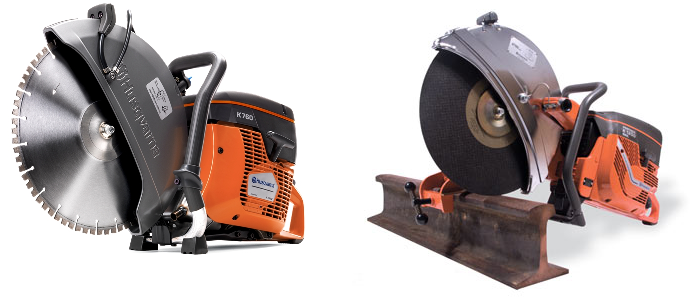
\includegraphics[width=0.9\textwidth]{img/k760-vs-k1260rail.png}
	\caption{K760 e K1260 RAIL}
	\label{fig:k700vsk1260}
\end{figure}

\begin{figure}[h!]
	\centering
	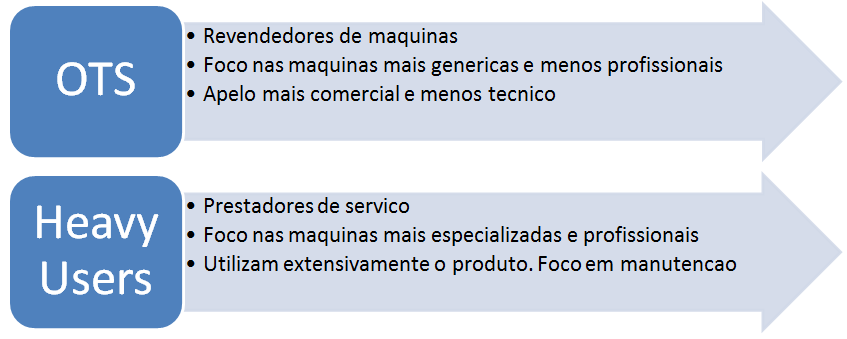
\includegraphics[width=0.9\textwidth]{img/clientes.png}
	\caption{Tipos de clientes}
	\label{fig:tipo-clientes}
\end{figure}

	O segundo grupo é conhecido como "heavy users" e corresponde aos prestadores de serviço de médio e grande porte. Esse público necessita de máquinas mais profissionais e robustas e os principais produtos consumidos são as serras mais pesadas, serras de chão, robôs de demolição e serras de parede. A decisão de compra, nesse caso, é mais focada nos aspectos técnicos do produto (custo de manutenção, potência, eficiência) e isso exige da Husqvarna um portfólio com soluções extremamente especializadas, que realizam determinados serviços com a maior eficiência possível. Os heavy users realizam serviços diversos de construção e em geral, utilizam o maquiário no dia-a-dia. A sofisticação dessa linha de produtos requer suporte e manutenção mais cuidadosos, pois alguns produtos tendem a ter mais de 400 horas de uso ao ano. 
	
	Na figura \ref{fig:k700vsk1260}, pode-se visualizar a diferença entre uma máquina genérica (à esquerda) e uma máquina especializada em cortar de trilhos de trem. A máquina especializada, apesar de executar apenas um tipo de serviço, o faz com melhor eficiência. Na figura \ref{fig:tipo-clientes} pode-se visualizar as pricipais características de cada grupo de clientes.
	


\subsection{Estrutura administrativa}


\subsection{Instalacoes}
Na Alemanha a empresa não possui plantas de produção, porém existe dois depósitos e um escritório de vendas. O escritório - responsável por toda a Alemanha - e um dos depóstitos estão localizados na cidade de Niederstotzingen, em Baden-Wurtemberg, à cerca de 100 km de Stuttgart. O segundo depósito fica na cidade de Mullheim, próximo à fronteira com a França.

Diante da ausência de planta de produçao no país, o número de funcionários na Alemanha é baixo. São menos de 50, que fazem todas as atividades de vendas, despacho, compras e afins.

\section{Teoria}

\subsection{Preco, Custo e Valor}
Existem alguns conceitos econômicos envolvidos em operações de venda que é imortante compreender, porém são normalmente confundidos entre si. São eles:

\subsubsection{Preco}
Preço é a quantidade de pagamento ou compensação dado por uma parte à outra em troca de produtos ou serviços. Na economia moderna, o preço é normalmente expressado em relação a uma moeda corrente. Juntamente com a definição de preço existe uma outra conhecida como Preço de Venda. Este nada mais é que o valor que uma parte pede à outra em troca de mercadorias ou serviços. O Preço de Venda pode ser diferente do Preço da Transação se, por exemplo, o vendedor der algum desconto.

\subsubsection{Custo}
Custo corresponde à quantidade de dinheiro utilizado para produzir algo. Os custos podem ser dividdos em fixos e variáveis. Custos variáveis são todos aqueles que estão diretamente ligados à produção de algo. Quanto maior a quantidade de itens prodruzidos, maior o custo variável. Por outro lado, os custos fixos são custos necessários para a produção de algo, mas que não variam com a quantidade de itens produzidos. Um exemplo de custo fixo é o aluguel de um galpão de fábrica.

\subsubsection{Valor}
O valor é muitas vezes confundido com o preço, pois normalmente é expressado em unidade de moeda corrente, porém trata-se de um conceito econômico que é definido por alguns fatores como: usabilidade intrínseca ao produto, a demanda que o mercado tem por este produto, bem como a sua oferta. É possível resumir o conceito de valor respondendo à seguinte pergunta: "Qual é o preço máximo que um cliente pagaria por este produto?".

Dentro do marketing existe um outro conceito chamado de Valor Percebido. Ele é, basicamente, a divisão entre o Valor de um produto e o seu Preço. O Valor Percebido é o que rege a ação de compra de um determinado consumidor. Quanto maior for o valor percebido, mais provável é que o consumidor efetue a compra de um produto ou serviço. Vale lembrar que o Valor Percebido não é simplesmente o valor econômico, mas sim algo mais subjetivo, que leva em conta questões como popularidade, grife, sazonalidade, etc.

Um exemplo simples da subjetividade do Valor é um pacote de café brasileiro vendido no Brasil e na Europa. Os clientes europeus veem um valor maior no produto (por ter vindo do Brasil) do que os clientes brasileiros. Se o pacote de café fosse europeu, essa relação de valor provavelmente se inverteria.

\subsection{Financas Corporativas}
O lucro líquido de uma empresa é definido como as entradas de capital menos as saídas, entretanto, existem outros indicadores intermediários que servem para outros tipos de análise. O cálculo desses indicadores não segue uma regra específica e apesar de todos eles terem uma regra geral, muitas vezes são realizadas algumas simplificações em fatores que não interferem tanto no resultado, seja por causa da análise a ser feita ou pelo tipo de negócio que a empresa faz. 

%(MOZINHO, ESSE PARÁGRAFO DE CIMA ESTÁ MUITO LINGUIÇADO. NÃO FICOU CLARO O QUE VC QUIS DIZER.)

\begin{figure}[h!]
	\centering
	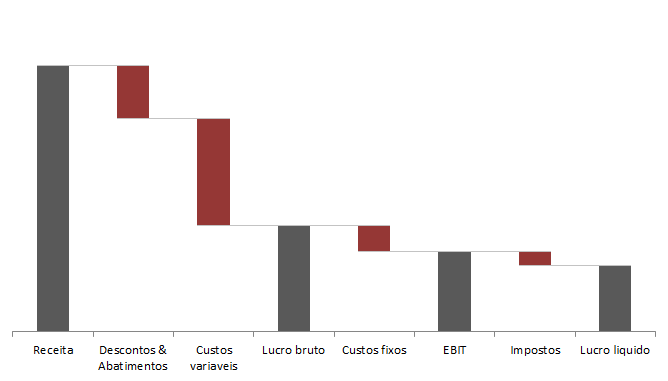
\includegraphics[width=0.9\textwidth]{img/finance.png}
	\caption{Representacao esquematica do calculo de lucro liquido}
	\label{fig:lucro}
\end{figure}

A figura \ref{fig:lucro} mostra uma das representações mais simples utilizadas para o cálculo do lucro líquido através de deduções da receita obtida pela empresa. Nos itens abaixo serão discutidos alguns dos indicadores intermediários, seus cálculos e utilização. 

\subsubsection{Receita}
Receita é a entrada monetária que ocorre dentro de uma empresa, normalmente relativa à vendas de mercadorias ou serviços. As receitas podem ser brutas ou líquidas e operacionais ou não-operacionais. A receita bruta é aquela que corresponde ao valor negociado na aquisição de um produto e é a utilizada para cálculo de impostos sobre ascvendas. A receita líquida então é a receita bruta descontada de devoluções, impostos diretos sobre o valor de venda e abatimentos.
A receita operacional é toda aquela proveniente da atividade principal de uma empresa, enquanto a receita não-operacional é resultado de atividades não principais da empresa. Um exemplo de receita não-operacional são aplicações financeiras.

\subsubsection{Desconto e Abatimento}
Desconto e abatimento são reduções no preço de um produto realizadas para determinados clientes ou grupo de clientes. A diferença básica entre desconto e abatimento é que o primeiro refere-se a uma redução realizada antes da emissão da nota fiscal, enquanto o segundo é realizado depois. Comumente os descontos são utilizados por empresas para incentivar um cliente a comprar determinado produto ou a não comprar um produto similar do concorrente. Abatimentos são utilizados para incentivar um cliente a comprar quantidades maiores de determinados produtos. As compras podem ser realizadas em datas diferentes e o cliente recebe um abatimento no valor da compra quando atinge uma determinada meta de volume.

\subsubsection{Custos Variaveis}
Custos variáveis são todos aqueles que têm relação direta com a quantidade produzida. Para uma indústria, os custos variáveis podem ser: matéria prima, mão de obra direta, energia elétrica direta, entre outros. Para o caso de um escritorio de vendas, os custos variáveis são o preço interno e o custo de transporte da fábrica até o depósito.

\subsubsection{Lucro Bruto}
Lucro Bruto corresponde à receita líquida menos os custo variáveis. Ele revela o quanto o produto gera de lucro, sem levar em consideração a estrutura administrativa e seus respectivos custos fixos.

\subsubsection{Custos Fixos}
Custos fixos sao todos os que nao são proprocionais ao volume produzido. Isso inclui o salário do setor administrativo, aluguel, energia utilizada em atividades não produtivas, etc.

%MOZI, ACIMA, VOLUME VENDIDO OU PRODUZIDO?
%produzido :D

\subsubsection{EBIT}
EBIT é a sigla em inglês para Earnings Before Interest and Taxes (Lucro antes de Juros e Imposto de Renda). Ele é correspondente ao lucro total obtido pela a empresa sem levar em conta a política de distribuição de lucros, juros de empréstimos anterioes, bem como impostos sobre o lucro. O EBIT tem duas finalidades: a primeira é enquanto indicador de como a empresa esta perfomando no presente - como este valor não leva em conta o pagamento de juros, o lucro da empresa do período não é punido por empréstimos que a empresa fez no passado; a segunda função é ter uma relação entre duas empresas distintas - como o EBIT desconsidera o pagamento de impostos, ele não está punindo uma empresa que encontra-se em um pais no qual os impostos são maiores. O EBIT também não considera a distribuição de lucros, ou seja, não pune uma empresa que distribui mais lucros para os seus acionistas.

\subsubsection{Impostos}
Impostos são a última dedução realizada antes do lucro líquido. O imposto dedudzido nesta etapa corresponde ao imposto sobre o lucro obtido.

\subsubsection{Lucro Liquido}
Lucro líquido é o capital que sobra para a empresa após cumprir todas as suas obrigacões fiscais e legais.

%PAREI AQUIIIIIIIIIII!!!!!
% <3

\subsection{Efeitos Financeiros}
Efeitos financeiros sao os impactos que ocassionam uma diferenca de financeira entre dois periodos. Sua maior utilizacao eh para quais foram as causas que trouxeram uma diferenca de lucro, rentabilidade, custo no periodo. Nao existe uma classificacao fixa para quais sao os efeitos financeiros, por regra, os mais utilizados para o calculo de diferenca de lucro sao: Volume, Preco, Custo e Mix.

\begin{figure}[h!]
	\centering
	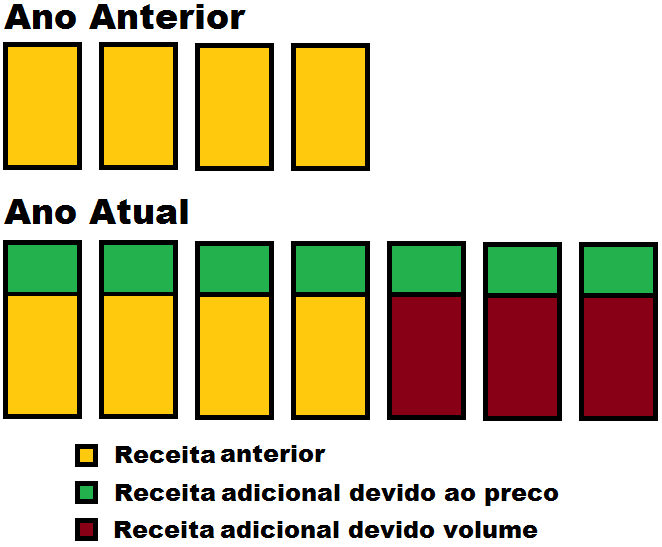
\includegraphics[width=0.6\textwidth]{img/effects.png}
	\caption{Representacao esquematica dos efeitos de volume e preco}
	\label{fig:effects}
\end{figure}

Na figura \ref{fig:effects} pode se ver uma representacao simples dos efeitos volume e preco na rentabilidade entre dois anos. Cada retangulo corresponde a 1 produto vendido e a sua area a rentabilidade total. No primeiro ano foram vendido 4 produtos. No ano seguinte, foram vendidos 7 produtos com um leve aumento de preco. A area em amarelo corresponde ao faturamento correspondende ao ano anterior. Em verde devido ao aumento de preco e em vermelho devido ao aumento de volume.

\subsubsection{Efeito Volume}
Corresponde ao lucro adicional ocasionado pelo aumento de volume de vendas.

\subsubsection{Efeito Preco}
\subsubsection{Efeito Custo}
\subsubsection{Efeito Mix}

\section{Projetos Realizados}

	O estagio foi realizado dentro do escritorio de vendas da Alemanha, as principais atribuicoes durante o estagio foram desenvolver projetos para aumentar algum indicador de vendas e ajudar em atividades do dia-a-dia.  Durante o periodo dois projetos foram de grande importancia e ajudaram a desenvolver areas da empresa que nao estavam bem desenvolvidas. O primeiro deles trata de uma nova metodologia para precificacao de pecas de reposicao, enquanto o segundo trata do desenvolvimento de um programa de manutencao para um dos produtos fabricados pela Husqvarna. Devido ao tempo do estagio, o segundo projeto se limitou apenas a uma maquina, mas o modelo de negocio escolhido pode ser utilizado para qualquer tipo de maquina.

\subsection{Politica de precificação para peças de reposição}

	Os equipamentos para construcao civil da Husqvarna sao focados no publico profissional. Isso significa que as maquinas devem ser desenvolvidas para uma alto numero de horas de uso (algumas chegam a ser utilizadas 400h por ano). Por esse motivo, falhas sao frequentes e a disponibilidade e preco das pecas de reposicao eh uma dos principais guia que fazem as empresas comprar as maquinas. O objetivo deste projeto eh analisar a precificacao que a Husqvarna e seus concorrentes fazem nas pecas de reposicao, bem como a maneira que o cliente avalia o "valor" de uma peca e montar uma estrategia de precos que aumente o faturamento da empresa e a satisfacao do cliente.

	Na maioria da empresas, a conta que se realiza para o calculo de preco eh basicamente utilizar o custo de determinado produto e adicionar uma margem esperada. O problema dessa abordagem eh que, nao levando em conta o preco do mercado, voce pode estar vendendo mais caro que o cliente quer pagar (perdendo assim volume) ou vendendo mais barato do que o cliente pagaria (perdendo assim lucro). A maneira ideal de se obter o preco de um produto eh fazer a analise inversa: Qual eh o preco maximo que o meu cliente estaria disposto a pagar por este produto? Atraves disso, voce pode descontar desse preco uma margem que vc considera interessante para a empresa e com isso ter o custo maximo que vc pode ter para esse produto ser rentavel.

	A husqvarna por ser uma empresa global tem um problema adicional. A diferenca de precos entre paises. A europa eh um continente onde os laços comerciais entre os paises sao muito fortes e eh facil para uma empresa analisar o preco de determinado produto no exterior. Por isso, os precos da Husqvarna devem fazer sentido nao soh para a Alemanha, como eles devem estar em linha com o que os outros paises cobram (Franca, Paises Baixos, Austria, etc). Eh normal os precos em determinado pais serem um pouco mais caro, mas isso deve se refletir para todo o portfolio de produto e nao apenas para 1 produto em especifico.

	Outro fator importante nessa analise eh o fato de muitos clientes (Heavy Users) possuem varias maquinas diferentes. Iss permite eles a fazerem comparacoes entre maquinas. Por exemplo, um cliente que possui uma serra grande e uma pequena, pode comparar os precos das pecas de reposicao. Ele pode entender o fato de um filtro de ar para uma maquina grande ser mais caro que um para uma maquina pequena, mas o contrario nao faz sentido. Neste caso, o cliente pode achar que o filtro para a maquina pequena esta muito caro.

	O primeiro passo desse projeto foi exatamente levantar esses problema e relizar um Brainstorming de solucoes. O fato da Husqvarna ser uma empresa grande torna o problema muito dificil de ser resolvido e eh esperado que nem todos os pontos e para todos os produtos podem ser resolvidos. A ideia do projeto, entretanto, eh pelo menos amenizar esses problemas.

\begin{figure}[h!]
	\centering
	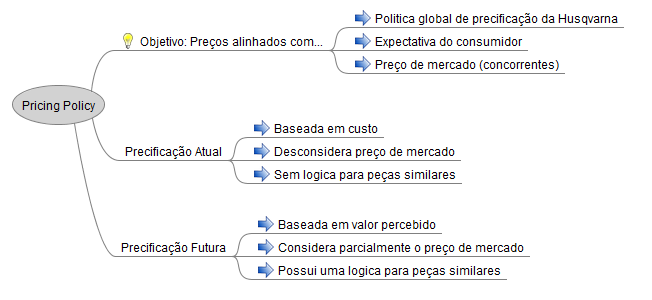
\includegraphics[width=0.9\textwidth]{img/pricing.png}
	\caption{Objetivos do projeto de precificacao}
	\label{pricing}
\end{figure}

	Historicamente os precos das pecas de reposicao eram calculados com base no custo. As margens de cada filial eram previamentes definidas e somando-se elas ao custo, obtia-se o preco final. O principal problema desse "approach" é que ele não leva em conta o preço de mercado. Simplesmente adicionando uma margem ao custo, não existe nenhuma garantia de que o produto sendo vendido tem um preço competitivo. Alem disso, essa visão não contribui para a redução de custos da empresa, tendo em vista que ela não consegue saber qual é custo "alvo" que deve buscar.

	O primeiro passo para corrigir esse problema foi trabalhar junto com a matriz em obter um preço internacional para cada produto. Como um primeiro balisador, obteve-se a média internacional de preços para cada produto. Observando esses preços, notou-se que eles apresentavam alguns problemas. 

	É conhecido que o custo de fabricação de um produto depende muito da quantidade produzida. Quanto maior a quantidade, menor o custo. O problema é que as máquinas mais vendidas pela Husqvarna são as máquinas menores (pois elas atendem tanto ao publico normal quanto o profissional) e por isso o custo de suas respectivas peças de reposição são menores do que as de maquinas maiores. Para o cliente final, a estratégia de produção da Husqvarna ou o seu portfolio de clientes não tem nenhuma relação com a decisão de compra. O cliente utiliza mecanismos mentais simples para tomar essas decisões. Por exemplo, para o cliente um motor de uma máquina menor deve ser necessáriamente mais barato do que o de uma máquina maior. Entertanto, devido a produção da Husqvarna, nem sempre isso acontecia.

	Para contornar esse problema, novos critérios tiveram que ser definidos para o cáculo do preço. Foi criado um índice chamado de "value driver" (TODO: preciso traduzir isso). O value driver é basicamente o parametro que o cliente enxerga como valor no produto. No caso de um motor por exemplo, utilizou-se a cilindrada. Quanto maior a cilindrada, maior o preço. No caso de parafusos, foi o peso. Quanto mais pesado e "heavy duty" um parafuso, mais caro ele era. A tabela XX mostra o value driver utilizado para alguns grupos de peca.

%COLOCAR TABELA AQUI!!!

	Atraves do value driver, foi possível melhorar a análise de preco. Os precos que eram antes apenas baseados em custo, agora não dependem mais da estrategia de producao da Husqvarna e fazem mais sentido para o cliente final. No entanto, isso não era suficiente. Para se obter um preco ainda melhor, foi necessario descobrir qual era o preço de mercado de cada produto.

	O preco de mercado corresponde a uma média de precos realizado por todos os players dentro de um mercado especifico. Com o objetivo de obter esse preco, realizou-se uma pesquisa de mercado. Essa pesquisa foi realizada atraves da obtencao de lista de preço de revededores multi-marcas, pedido de cotação enviado para revendedores de concorrentes e através do "input" do time de vendas. Utilizando os dados obtidos, realizou-se um ajuste dos precos ja calculados.

	Outro fator importante sobre precificacao eh que ela nao pode ser realizada em movimentos bruscos. para isso foi definidida uma taxa arbitraria de 3\% para a mudanca de preco. Entretanto, alguns artigos seguiram uma regra diferente.

	Para os artigos com um preco muito baixo, parafusos por exemplo, uma mudanca de 100\% corresponde a poucos euros, o que de certa forma nao afeta o consumidor final. Seguindo essa teoria, foi determinado que todos os artigos com o preco atual e alvo menor do que 10 euros seria modificado diretamente para o preco alvo.

Outro fator importante eh que o cliente soh tem a possibilidade de comparar o preco historico de pertes que ele ja comprou. Por isso foi criada uma nova categoria de produtos que nao tiveram vendas desde 2011. Esse produtos tambem foram modificados para o preco alvo.

Por ultimo, foram detectado alguns precos que estavam totalmente fora da realidade. Provavelmente produtos onde houve erro de digitacao no preco. Para esses produtos tambem se realizou a correcao diretamente para o alvo.

\subsection{Serviço de manutenção de serras de parede}

\begin{figure}[h!]
	\centering
	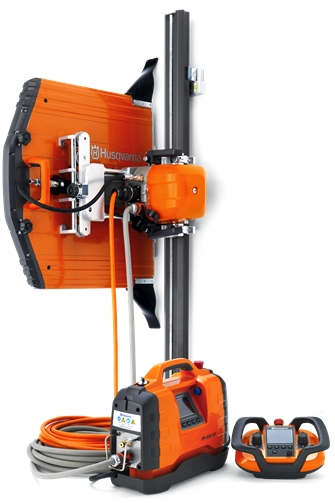
\includegraphics[width=0.4\textwidth]{img/ws220_produto.png}
	\caption{Serra de parede modelo WS220}
	\label{fig:ws220_produto}
\end{figure}

	Para um empresa prestadora de serviços de construção na Alemanha os gastos referentes a aquisição e manutenção das ferramentas de trabalho correspondem a um valor expressivo do custo total da empresa. Além disso o ambiente agressivo e o uso constante no qual as maquinas são expostas são motivos frequentes de falhas até mesmo nas máquinas mais robustas. Para um empresa menor que possui poucas máquinas a falha de uma delas pode ter consequencias devastadoras. Além dos custos de reparo, os dias em que a empresa fica impossibilitada de trabalhar gera um grande impacto negativo no fluxo de caixa.

	O objetivo do projeto era desenvolver um pacote de manutenção para transferir o risco de fluxo de caixa do cliente para a Husqvarna. Uma venda suficientemente grande de pacotes de manutenção para a Husqvarna é uma boa maneira de mitigar o risco de fluxo de caixa, tendo em vista que apesar das falhas serem imprevissiveis é possível a empresa calcular uma média de gastos anuais. Com um número suficientemente grande de máquinas a probabilidade que as falhas ocorram no mesmo mês é extremamente baixa. Para esse projeto específico, foi escolhida uma serra de parede modelo WS220. O motivo da escolhe deve-se ao fato que esse modelo é lançamento no mercado e por isso é mais fácil apresentar novidade aos clientes.

	Utilizando a metodologia do Balance Scorecards, o projeto foi divido em etapas, onde cada etapa corresponde a um fator crítico de sucesso. Os fatores do BSC podem ser visualizados na figura \ref{fig:bsc}. Para o quesito Financeiro foi definido a realização de uma análise de custos do produto; Para o fator Cliente, foi realizada uma análise na questão de precificação do produto e serviços; Na questão de Processos Internos foi desenvolvida toda a documentação em relação ao pacote. De forma que a aplicação desse projeto seja realizada de forma fácil e correta dentro da empresa; Por último, na questão Aprendizagem e Crescimento, foi criada uma documentação do projeto de forma que a replicação para outros produtos seja relativamente fácil. Na figura \ref{fig:service} pode-se ver uma analise geral das questões a serem respondidas pelo projeto.

\begin{figure}[h!]
	\centering
	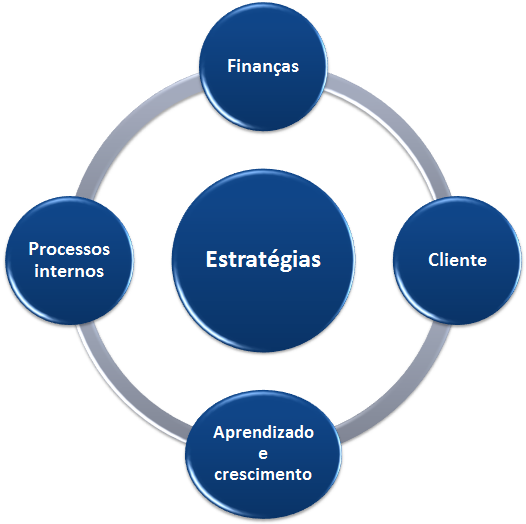
\includegraphics[width=0.4\textwidth]{img/bsc.png}
	\caption{Matriz BSC}
	\label{fig:bsc}
\end{figure}

\begin{figure}[h!]
	\centering
	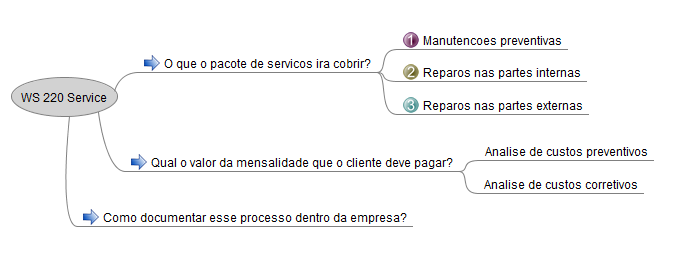
\includegraphics[width=0.9\textwidth]{img/ws220.png}
	\caption{Objetivos do projeto de servico}
	\label{fig:service}
\end{figure}

\subsubsection{Analise de custos e precificacao}

	Para o custo de manutenção preventiva, utilizou-se o manual de reparos do produto para efetuar uma lista de serviços de manutenção que devem ser realizados a cada intervalo de tempo. Com base nesses dados foi calculado o custo desses serviço com base no preço interno. Além disso, o custo da mão-de-obra foi determinado pelo time de manutenção. Com base nos serviços que devem ser realizados, o time deu uma estimativa de horas para completar. Com base nessa estimativa e no custo de uma hora de trabalho foi estimado o custo de mão-de-obra.

\begin{figure}[h!]
	\centering
	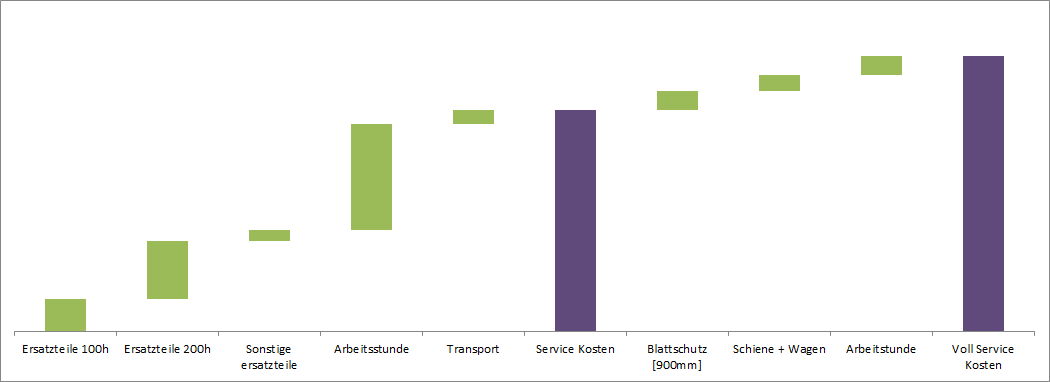
\includegraphics[width=0.9\textwidth]{img/ws220-waterfall.png}
	\caption{Calculo de custos do projeto}
	\label{fig:ws-waterfall}
\end{figure}

	Em relação a análise de custos, primeiramente foi obtido os dados de taxa de falha para cada componente da máquina. Esses dados correspondem a média de produtos que apresentam falha a cada 100 horas de uso. Esses dados foram então extrapolados para uma população de mil produtos e 500 horas de uso e o custo total de reposição das peças que apresentaram falha calculado com base no preço interno + frete. Esse custo corresponde ao custo de manutenção corretiva. A mão-de-obra foi calculada utilizando o custo das peças e a estimativa da manutenção preventiva. na figura \ref{fig:ws-waterfall} pode-se visualizar os dados finais da analise de custo (os valores foram removidos do grafico por serem dados confidenciais). O custo total de manutenção é a soma dos custos de manutenção preventiva, corretiva e transporte da máquina. Com base nesse custo foi possível adicionar a margem de lucro da empresa e obter o preço final para o cliente.
	
\subsubsection{Documentacao externa e interna}

	Seguindo a analise do BSC, para os quesitos de Processos Internos e Aprendizagem e Crescimento, foram desenvolvidas documentacoes externas e internas.

\pagebreak

\section{Observacoes referentes as informacoes do relatorio}
	Algumas informações como dados financeiros, estrategias de marketing e dados sobre produtos são consideradas sigilosas e, portanto foram omitidas neste relatório devido á política de sigilo da Husqvarna.
\pagebreak

\section{Considerações finais}
\pagebreak

\end{document}
